\chapter{Sketch Simplification}

Sketch Simplification refers to automatically converting rough sketches into simplified clean drawings. It is one of the most fundamental tasks because it is the first step in the whole pipeline. An accurate and fast method is required to provide a solid foundation for subsequent processing. However, as we will see, it is a relatively under-explored area and we have yet to see a fast and high-quality procedure for this task. Nevertheless, the task itself is relatively straight forward and similar problems have developed mature solutions, therefore it is not expected to be difficult. I will explain the recent research and main challenge and possible future direction in the following sections.

\label{chapterlabel4}
\section{Approaches \& Methods}
Traditionally, rough sketches are iteratively refined by the artist himself/herself. This requires manually tracing the rough sketch repeatedly to produce a clean and satisfying drawing. This process is tedious, time-consuming and involves a large overhead. There have been some methods proposed to simplify sketch drawings. Some assists user to clean up sketches based on geometry relationships between strokes\cite{fiserShipShapeDrawingBeautification2015} and fitting stroke using Bezier Curves\cite{baeILoveSketchAsnaturalaspossibleSketching2008}; Others simplify rough lines by removing unnecessary ones\cite{liuClosureawareSketchSimplification2015}. However, these traditional methods neither change the way artists clean up sketches nor provide a fully automatic way to simplify them. Moreover, they often operate on vector graphics, which is more dominant in the design industry and not the 2D animation industry.

\begin{figure}
    \centering
    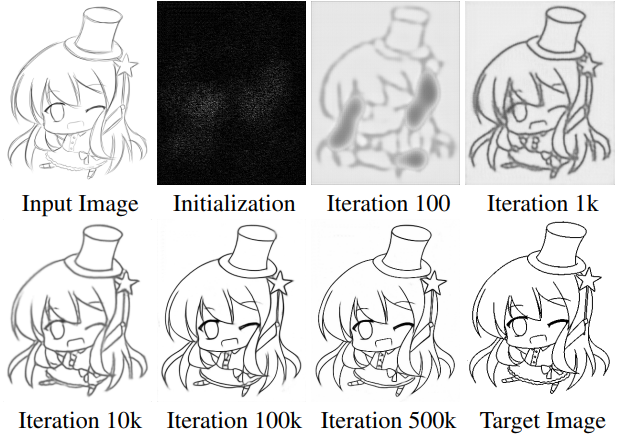
\includegraphics[width=0.75\textwidth]{images/sketch/learning2simp.png}
    \caption[Visualization of the output image as training proceeds for encoder-decoder CNN model.]{Visualization of the output image as training proceeds for encoder-decoder CNN model. As iterations increase, the cleaned sketch gradually becomes more clear and more polished. The model initially focuses on joining multiple lines into one and producing a rough structure; later focuses on details and is able to simplify the lines and converges. Note that it took 500k iterations for this image to converge, which is very high and this means a long training time that is probably prone to some over-fitting issues.\cite{simo-serraLearningSimplifyFully2016}}
    \label{fig:learning2simp}
\end{figure}

Later some algorithmic approaches are proposed, most of which convert the image into a graph and apply optimization techniques\cite{favreauFidelityVsSimplicity2016}. However, the graph representation often generates unrecoverable errors because images often consist of a large number of isolated graphs and connections between them are hard to model. Other approaches convert the raster image into a vectorized image, fit and merge Bezier Curves based on heuristics\cite{fiserShipShapeDrawingBeautification}. Such conversion does not generate unrecoverable errors but requires additional input such as the order of the strokes drawn in the raster image which typically does not exist in our context.

\begin{figure}
    \centering
    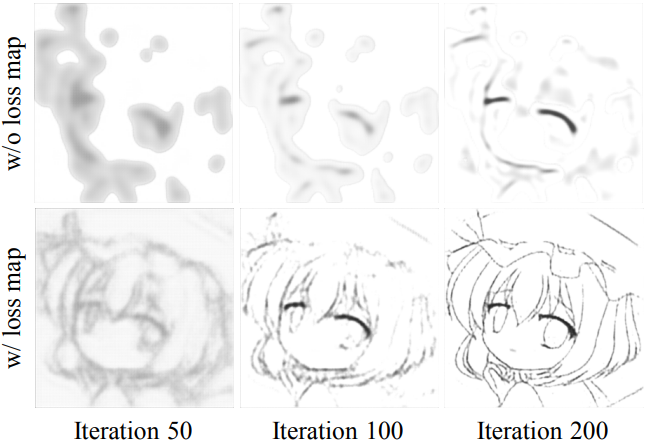
\includegraphics[width=0.75\textwidth]{images/sketch/loss-map-compare.png}
    \caption[Speed of convergence with and without loss map.]{Speed of convergence with and without loss map. We can observe that with the same number of iterations, the use of a loss map significantly increases the quality of the output image.\cite{simo-serraMasteringSketchingAdversarial2017}} 
    \label{fig:loss-map-compare}
\end{figure}

As far as I know, the first attempt to simplify sketches in a fully automatic way on raster images was in 2016\cite{simo-serraLearningSimplifyFully2016}. The researchers used an encoder-decoder CNN architecture and achieved reasonable results. Worth mentioning, they used a loss map which assigns a higher weighting to lines and achieved much faster training (see figure \ref{fig:loss-map-compare}). Their results showed that for simple sketches the model can produce accurate strokes (see figure \ref{fig:learning2simp}). Follow-up research approached this problem with a simple cGAN model and achieved slightly better results\cite{simo-serraMasteringSketchingAdversarial2017}, and was able to handle the inverse problem by converting clean sketch to rough sketch. Both attempts only trained with 68 pairs of data, which is insufficient, prone to bias, and does not prove the generalization capability of the model. But we have no way of knowing because they did not disclose the dataset used, and there are no other known attempts  to convert rasterized rough sketch to rasterized clean sketch directly that has a similar context to this master project.

Figure \ref{fig:sketch-simp-works} compared various techniques proposed for simplifying sketches in recent years. We can see that the graphical method produced unnatural segmentations, resulting in unpleasant sketches. The deep-learning-based method offered much more natural results, but many details are ignored by the model. The encoder-decoder approach created a much more abstract representation, signalling the authors were not reserving enough latent space. Nevertheless, it produces more eye-pleasing results than the graph-based method. The GAN-based method produced noticeably more details and ignored more unrelated strokes which made it performs better than others.

\begin{figure}
    \centering
    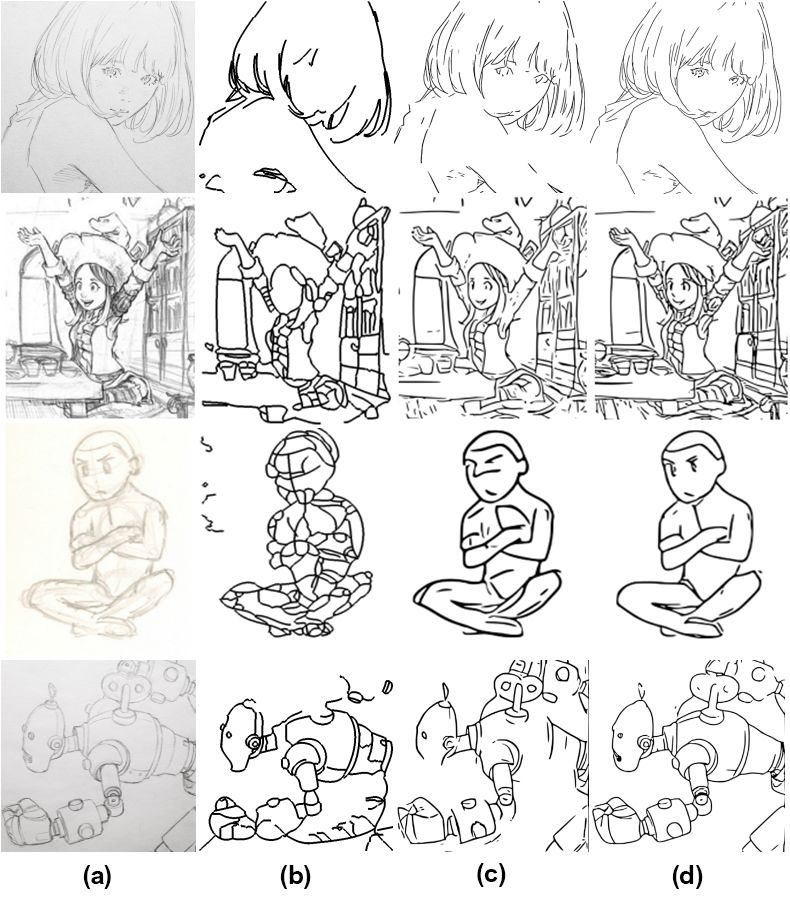
\includegraphics[width=1.0\textwidth]{images/sketch/sketch-simp-works.png}
    \caption[Comparison of different sketch simplification results.]{Comparison of different sketch simplification results. Column (a) is the input image; (b) is the results from the graphical optimization method; column (c) is the results from encoder-decoder CNN architecture; column (d) is the results from vanilla GAN architecture. The graphical method generated unpleasing segmentations, the encoder-decoder method encoded many unnecessary details and the GAN approach is able to capture the overall structure and skip un-relevant details. We can observe that there is an increase in the number of details going from left to right.\cite{simo-serraMasteringSketchingAdversarial2017}}
    \label{fig:sketch-simp-works}
\end{figure}

All aspects of the model: preprocessing, augmentation, architecture and training etc. are simple without many modern techniques, however, they can generate relatively precise results. This showed that this task is comparatively simpler than others. However, the main challenge lay in this task is the training data. It is difficult to find high-quality training samples and papers either do not disclose the dataset they use or it is not suitable for our task. For example, there exists a benchmark dataset for sketch simplification\cite{yanBenchmarkRoughSketch2020}. However, this dataset focus on removing shadows and composition guidelines from the sketch image, rather than converting rough lines into clean lines.

There exist attempts to tackle the inverse problem of translating cleaned sketches into rough sketches, however, generated sketches often lack properties that exist in real rough sketches, producing a hard-to-generalize result\cite{simo-serraMasteringSketchingAdversarial2017}. Therefore the researches are not up to the standard for us to generate synthetic data.

Another problem that is worth mentioning is most papers do not mention the high amount of training iterations used despite a small amount of training data. For example, the SOTA model\cite{simo-serraMasteringSketchingAdversarial2017} uses only 68 pairs of supervised data trained for 150k iterations. There are two explanations for this: (1) the results are overfitting, and (2) it is hard to refine the network to a plausible and stable state. Overfitting is unlikely because if it is overfitting, it will happen much sooner and results in a more aggressive similarity. The latter is much more probable, this is because the sketch itself contains only very sparse information and the line difference between clean and rough ones may be indistinguishable after a few convolutional, and more general details are being extracted rather than these details. Therefore it takes a long training time for the model to focus on what is important. On the other hand, this also reflects the inefficiency of the loss function used in current research. We can see that the use of GAN did improve the training time, from 350k\cite{simo-serraLearningSimplifyFully2016} in a similar setting to 150k\cite{simo-serraMasteringSketchingAdversarial2017}. However, the iterations per sample ratios are still very high, which can cause trouble in training larger-scale models.

\section{Design \& Implementation}
\subsection{Dataset}
Both input and output are binary grayscale images. Due to the lack of a high-quality dataset, I adopted the dataset from NoGhost. Due to the limited amount of training data, extensive augmentation is used, this includes random horizontal flip, random rotation, and random resized crop. Additionally, with a probability of 10\%, the input is set to the target image to encourage the model not to change any cleaned sketches. The images are normalized with a mean and variance equal to $0.5$ for more stabilized input. The final dataset contains around 400 pairs of training and testing data.

\subsection{Models}
The model follows a pix2pix architecture, where the generator is a U-Net generator and the discriminator consists of a stack of convolution layers. The U-Net generator consists of 6 pairs of up and down scaling blocks, the number of channels in each block is $32, 64, 128, 256, 512, 1024$. Drop out with probability $50\%$ are added to the output of the 2 innermost blocks in the U-Net. The discriminator consists of 5 convolutional blocks, each consisting of a convolution layer, followed by batch normalization layer, and leaky ReLU layer. The number of channels of the convolution layers is $256, 128, 64, 32, 16$. A sigmoid activation is added at the end of the model.


\subsection{Training}
Training parameters are batch size = 8, epochs = 500, learning rate = 0.0002, image size = 512. In addition, the training rate is gradually reduced to 0 during the last 100 epochs of the training. Optionally, a weight map can be used to speed up training. Weight map refers to assigning more weights to target image strokes to the output image when calculating its loss. This asks the model to focus on these areas and can speed up training, Additionally, its dilation variant can also be used. These techniques are compared in the following paragraphs. 

\section{Analysis}

We will first analyse the impacts of using various techniques on the structure of the image before diving into the quality of detail. This is because as we have observed from existing research, finetuning details requires a large amount of time. To be precise, in order to achieve similar iterations/samples used in the above papers using the NoGhost dataset, it would take 2-3 days to train one model using GoogleColab. Therefore following analysis' results are trained with  $\frac{1}{4}$ of the target iterations.


\subsection{Vanilla vs Weight Map vs Dilated Weight Map}
\begin{figure}
    \centering
    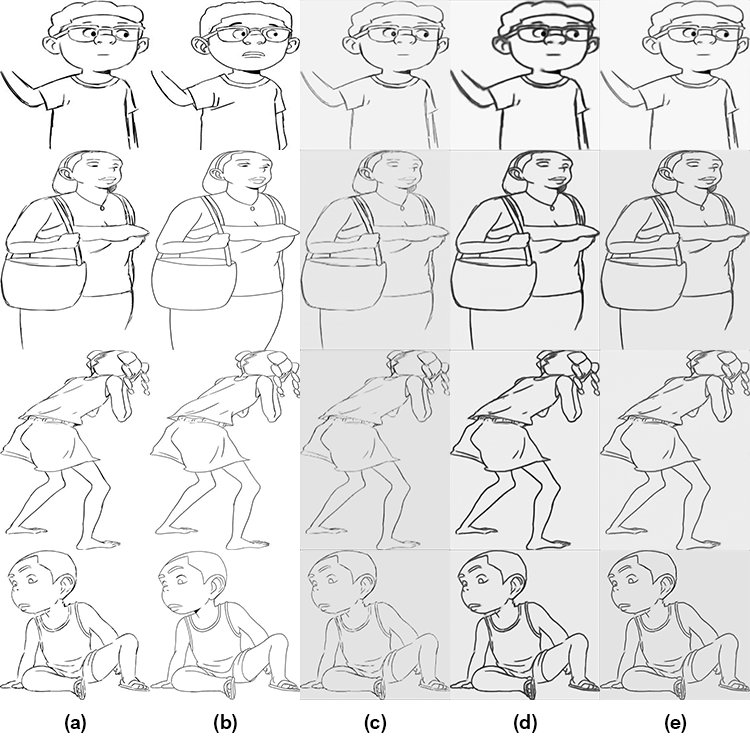
\includegraphics[width=1.0\textwidth]{images/sketch/dilates_comparison.png}
    \captionsetup{singlelinecheck=off}
    \caption[Comparison of result using different types of weight map methods.]{Comparison of result using different types of weight map methods.
    \begin{itemize}
        \item \textbf{(a)} is input image.
        \item \textbf{(b)} is target image. 
        \item \textbf{(c)} is output without weight map.
        \item \textbf{(d)} is output with weight map.
        \item \textbf{(e)} is output with dilated weight map.
    \end{itemize}
    We can observe output without a weight map seem to be less confident about its output, more discontinued lines and lower output values. Other the other hand, output with a weight map seems to be over-confident with its output, outputting high values across the weighted area, this results in generating thicker lines than it is supposed to. Output with dilated weight map has more appropriate contrast and outputs the cleaner lines than others.
    }
    \label{fig:dilates_comparison}
\end{figure}

It has been mentioned that the use of a weight map can speed up training significantly. However, I found that the weight map itself can result in unwanted artefacts caused by over-confidence. Therefore some dilation was applied on the weight map we compare the outputs and found that it produced cleaner results (see figure \ref{fig:dilates_comparison}). This is because rather than focusing on the sketch strokes themselves, adding dilation encourages the model to also focus on the regions around the strokes, resulting in a more accurate boundary.

\subsection{L2 Loss vs L1 Loss}
\begin{figure}
    \centering
    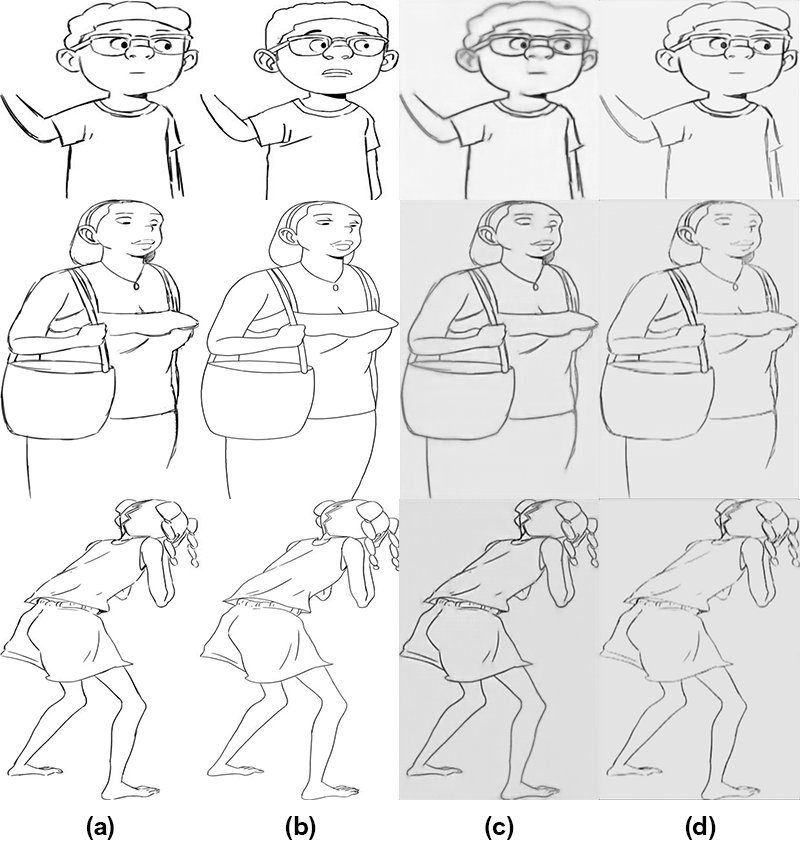
\includegraphics[width=0.75\textwidth]{images/sketch/l1_vs_mse.png}
    \caption[Comparison of results trained using L1 loss and L2 loss.]{Comparison of results trained using L1 loss and L2 loss.\textbf{(a)} is input image, \textbf{(b)} is target image, \textbf{(c)} is output trained using L2 loss, and \textbf{(d)} is output trained using L1 loss.
    We can see that although L1 loss indeed produced a sharper image, it is not necessarily better in all aspects. For example, L1 loss removes many details and can potentially result in discontinued boundary, as we have seen in the previous colourization section, this can result in issues such as colour bleeding. However, blurriness is also not desired generally as it means the network is not confident in its decision-making, resulting in a less generalizable model.}
    \label{fig:l1_vs_mse}
\end{figure}

It has been commonly known that L2 loss can result in blurry output images as it minimizes the averaged error instead of the absolute error\cite{isolaImagetoImageTranslationConditional2018}. However, may not necessarily be plausible in our case because it can lead to discontinued lines (see figure \ref{fig:l1_vs_mse}), which, as we have mentioned in the colourization section, makes the subsequent colourization task vulnerable to colour bleeding issues. However, further research is required to investigate their relationship using a larger-scale dataset.

\subsection{Vanilla vs Content Loss}
\begin{figure}
    \centering
    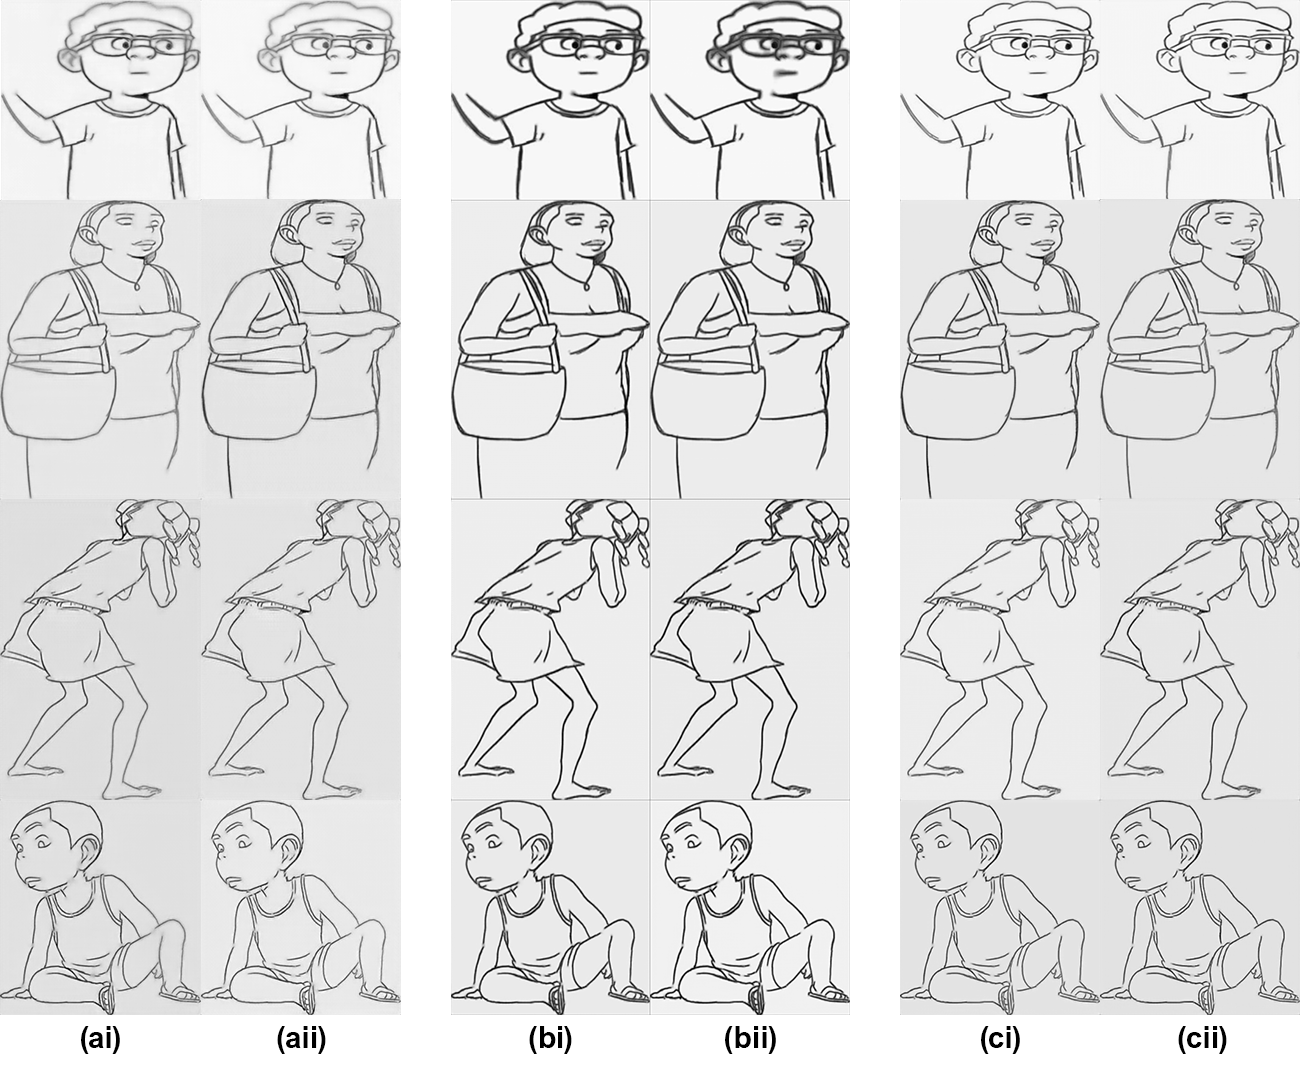
\includegraphics[width=1.0\textwidth]{images/sketch/content_loss_compare.png}
    \caption[Comparison of results trained with and without content loss under different settings.]{Comparison of results trained with and without content loss under different settings. \textbf{i} is output image without content loss and \textbf{ii} is output image with content loss. \textbf{(a)} is trained with L2 loss, \textbf{(b)} is trained with L2 loss + weight map, \textbf{(c)} is trained with L2 Loss + dilated weight map. We can see that the pairs are very similar. There is no clear distinction of which had produced cleaner lines.}
    \label{fig:content_loss_compare}
\end{figure}
As we have observed, the large number of training iterations could potentially be due to the ineffectiveness of the loss function. Therefore I experimented with the use of content loss to see if a pre-trained feature extractor could be used to speed up the training process. The pre-trained feature extractor I used is the $6^{th}$ layer of the vgg16 network pre-trained on over 12 million images. Figure \ref{fig:content_loss_compare} showed the training under various settings. It can be easily observed that the output samples are very similar and did not show significant improvements. Therefore we can conclude that the feature extractor did not extract much more useful information compared to the discriminator of the GAN model.

\section{Future Directions}
The current state of sketch simplification is the most research hungry out of all four tasks. It is a straightforward but hard-to-train. As we have seen from the above analysis, this is mostly due to: (1) difficulty in obtaining a high-quality dataset,  (2) difficulty in learning to refine the details, and (3) difficulty in designing a loss function. These three issues could potentially collapse into one. This is because problem (2) and (3) are consequent to problem (1). 
The presence of extra lines in the clean sketch forces the model to remember and focus more on these areas. This is because extra lines occupy a larger area than the rough sketch itself, resulting in a much greater loss thus, the model devotes greater effort to changing these areas, but it is futile since there is no reliable information provided to produce these extra lines. Moreover, this can contribute to overfitting.


